\documentclass{article}
\usepackage[preprint]{neuripsstyle}

\usepackage[T1]{fontenc}
\usepackage[utf8]{inputenc}
\usepackage{amsmath,amssymb}
\usepackage{booktabs}
\usepackage{graphicx}
\usepackage{microtype}
\usepackage{xcolor}
\usepackage{natbib}
\usepackage{tikz}
\usetikzlibrary{positioning,arrows.meta,calc,decorations.pathreplacing}
\usepackage[colorlinks=true,allcolors=black,citecolor=blue!55!black,linkcolor=blue!55!black]{hyperref}
\usepackage[capitalize,noabbrev]{cleveref}

\definecolor{cexec}{HTML}{D9D9D9}
\definecolor{cmaskc}{HTML}{F7D08A}
\definecolor{ceditc}{HTML}{A9CCE8}
\definecolor{cholec}{HTML}{FBF0B2}

\newcommand{\tinv}{\tau_{\mathrm{inv}}}
\newcommand{\thole}{\tau_{\mathrm{hole}}}

\title{Repair, Don't Replan: A Controlled Study of\\Observation-Conditioned Remasking in Masked-Diffusion Planners}

\author{%
  Anonymous Author(s)\\
  Affiliation\\
  \texttt{email@domain}
}

\noticeline{Workshop submission. All results are from the controlled synthetic testbed described in
\Cref{sec:env}; see \Cref{sec:scope} for scope and \Cref{sec:limits} for limitations.}

\begin{document}
\maketitle

\begin{abstract}
Masked-diffusion language models (dLLMs) can in principle edit a plan \emph{in place}: when a tool
observation invalidates part of a multi-step plan, the denoiser can remask exactly the affected
tokens and re-denoise them jointly with the surviving plan. Existing remasking methods are
\emph{introspective} --- they revise tokens the model itself judges low-quality --- whereas an agent
must revise tokens the \emph{environment} has invalidated. We isolate this setting in a controlled testbed --- 8-step tool plans, dataflow arguments,
state-diff success, mid-episode perturbations, small masked-diffusion and autoregressive (AR)
planners trained from scratch --- in which the ground-truth invalidation set is computable. Three findings. (i) At matched
success on in-distribution repairs, selective remasking regenerates $1.9$ tokens per episode versus
$83$--$84$ for full or AR-suffix replanning, using $27$ versus $108$ network calls; a
posterior-rescoring masker matches the oracle repair almost exactly (precision $0.92$, recall
$0.90$). (ii) On compositionally novel perturbation pairs held out from training, every learned
agent degrades ($0.75$--$0.88$) while the \emph{same} denoisers with oracle masking retain $0.996$:
localization, not repair synthesis, is the bottleneck, and the failure concentrates entirely in
repairs governed by an undemonstrated priority rule --- and a controlled intervention closes it:
adding just \emph{eight} demonstrations of that rule to training repairs the composed conditional on
every seed ($0.41\!\to\!0.997$), where ten-fold more single-perturbation repair supervision does
not. (iii) Outcome-reward RL restores repair from
supervision-scarce SFT on every seed ($\to 1.000$) yet composes worse than demonstrations; the naive
one-step policy gradient collapses, for a reason we identify. These are mechanism-study results on a
synthetic environment with $\sim$250k-parameter models, not a claim about 7--8B dLLMs.
\end{abstract}

\section{Introduction}

Diffusion language models are marketed on throughput, but a recent reality check finds they fail as
agentic backbones: on AgentBoard and BFCL, LLaDA and Dream repeatedly retry actions instead of
branching under temporal feedback and lose symbolic precision (e.g.\ strict JSON schemas) under
diffusion noise, with embodied success rates below 2\% \citep{bitterlesson2026,llada2025,dream2025}.
That work names \emph{diffusion-native agents} as the open direction. The strongest argument for such
agents is not speed but \textbf{editability}: an AR model that discovers at step 2 that its step 6 is
invalid can only append or regenerate a suffix, whereas a masked denoiser can return step 6 to
\texttt{[MASK]} and re-denoise it jointly with the surviving plan, preserving valid \emph{later}
steps and their dataflow bindings.

Whether that promise is real is not obvious. ``AR must replan'' is a strawman: an AR model can be
prompted to patch its plan, and prefix caching makes suffix regeneration cheap. Meanwhile most remasking work is
introspective --- RemeDi learns per-token confidence \citep{remedi2025}, ReMDM remasks on an
inference-time schedule \citep{remdm2025}, CoRe flags context-brittle tokens \citep{core2026}, with a
rapid stream of follow-ups refining the same signal
\citep{t2m2026,revise2026,selfcorrect2026,hong2025unmask}, and \citet{cdlm2025} show that standard
MDLM training does not even induce the ability to \emph{recognize} incorrect visible tokens.
Externally-triggered revision has begun to appear: \citet{zou2026detect} repair outdated spans of a
summary when the underlying document stream evolves. What remains unexamined --- and what we are not
aware of prior work evaluating --- is observation-conditioned remasking for \emph{temporally
unfolding tool-use plans}, where each executed step returns feedback, repairs must respect dataflow
across turns, and a ground-truth invalidation set exists to score localization itself. And at 7--8B
scale the confounds (weak base policy, JSON validity, RL instability) are entangled enough that a
negative end-to-end result would say little about the mechanism.

We therefore study the mechanism where it can be measured. We build \textbf{ToolFlow}, a synthetic
tool-use environment with 8-step plans, dataflow variables, state-diff success, and perturbations
revealed by observations mid-episode --- and, critically, a computable \emph{oracle invalidation
set}, which turns ``how good is the masker?'' into a precision/recall question and lets us separate
repair \emph{localization} from repair \emph{synthesis}. We train small masked-diffusion and AR
planners from scratch (identical architecture, bidirectional vs.\ causal), and compare five repair
strategies plus an AR-patch baseline across 5 seeds.

\paragraph{Contributions.}
(1) A controlled testbed for observation-conditioned plan repair with an oracle invalidation set and
a \emph{compositional} generalization split: training episodes contain at most one perturbation,
evaluation includes never-demonstrated perturbation \emph{pairs}.
(2) A head-to-head of repair strategies under matched success, with masker precision/recall, showing
selective remasking obtains oracle-sized repairs ($1.9$ tokens) at $\sim$44$\times$ less
regeneration than replanning and $4\times$ fewer network calls than an AR agent.
(3) The central diagnostic: with oracle masking the same denoisers execute novel composed repairs at
$0.996$, so the compositional gap is localization; per-family analysis pins the entire failure on
repairs governed by a priority rule absent from training; a supervision-dose intervention (\Cref{app:dose}) shows
eight demonstrations of that rule suffice to fix it while ten-fold more single-perturbation
supervision does not.
(4) A post-training study on a supervision-scarce start with the controls the claim requires: a
continued-SFT arm shows most of the gain is supervised, an isolated negative-advantage arm reproduces
the collapse of the naive one-step estimator, and we correct our own earlier mechanistic account
(\Cref{app:rl}).

\paragraph{Scope.}\label{sec:scope}
Every number here comes from a synthetic environment and $\sim$250k-parameter models trained from
scratch on one CPU core. We make no claim of quantitative transfer to 7--8B dLLMs on Agent-Diff
\citep{agentdiff2026} or BFCL \citep{bfcl2025}. We claim the mechanism is implementable, its
efficiency advantage is real under matched success here, and its failure mode is structured and
diagnosable. \Cref{sec:limits} states what does not follow.

\begin{figure}[t]
\centering
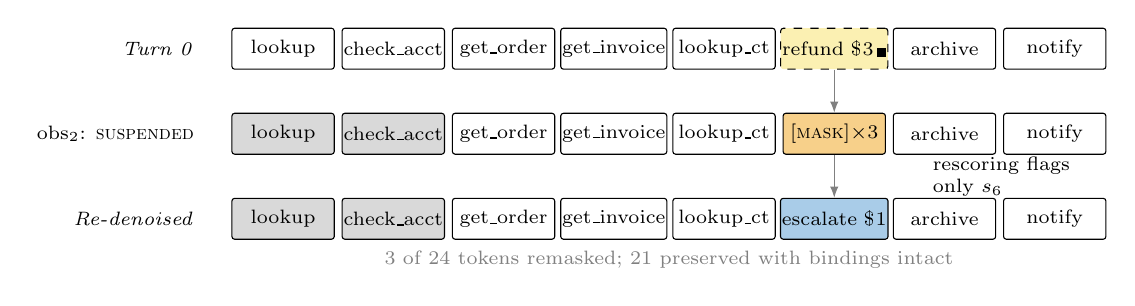
\begin{tikzpicture}[x=1.40cm, y=0.80cm, font=\scriptsize,
  cell/.style={draw, rounded corners=1pt, minimum width=1.30cm, minimum height=0.52cm,
               inner sep=0.5pt, align=center, line width=0.4pt},
  rlab/.style={anchor=east, font=\scriptsize}]

\node[rlab] at (0.28,0) {\emph{Turn 0}};
\foreach \i/\t in {1/lookup,2/check\_acct,3/get\_order,4/get\_invoice,5/lookup\_ct,7/archive,8/notify}
  {\node[cell] (a\i) at (\i,0) {\t};}
\node[cell, fill=cholec, dashed] (a6) at (6,0) {refund \$3\,\rule[-0.2ex]{1.1ex}{1.1ex}};

\node[rlab] at (0.28,-1.35) {obs$_2$: \textsc{suspended}};
\foreach \i/\t in {1/lookup,2/check\_acct}
  {\node[cell, fill=cexec] (b\i) at (\i,-1.35) {\t};}
\foreach \i/\t in {3/get\_order,4/get\_invoice,5/lookup\_ct,7/archive,8/notify}
  {\node[cell] (b\i) at (\i,-1.35) {\t};}
\node[cell, fill=cmaskc] (b6) at (6,-1.35) {[\textsc{mask}]$\times 3$};

\node[rlab] at (0.28,-2.7) {\emph{Re-denoised}};
\foreach \i/\t in {1/lookup,2/check\_acct}
  {\node[cell, fill=cexec] (c\i) at (\i,-2.7) {\t};}
\foreach \i/\t in {3/get\_order,4/get\_invoice,5/lookup\_ct,7/archive,8/notify}
  {\node[cell] (c\i) at (\i,-2.7) {\t};}
\node[cell, fill=ceditc] (c6) at (6,-2.7) {escalate \$1};

\draw[-{Latex[length=1.4mm]}, gray] (a6) -- (b6);
\draw[-{Latex[length=1.4mm]}, gray] (b6) -- (c6);
\node[font=\scriptsize, anchor=west, align=left] at (6.75,-2.03)
  {\;rescoring flags\\ \;only $s_6$};
\node[font=\scriptsize, gray] at (4.5,-3.35)
  {3 of 24 tokens remasked; 21 preserved with bindings intact};
\end{tikzpicture}
\caption{\textbf{Observation-conditioned selective repair.} A plan of 8 steps ($3$ tokens each) is
drafted at turn 0; the refund code is left as a \emph{typed hole} (dashed) because the tier is only
revealed at step 3. Executing step 2 returns \textsc{suspended}, which invalidates step 6 only. The
masker returns that step to \texttt{[MASK]} and the denoiser re-denoises it jointly with the intact
plan. Full replanning would remask all 18 downstream tokens; an AR agent would regenerate the
suffix. The showcase in Family B (\Cref{sec:env}) is harder still: steps 3 \emph{and} 7 change while
step 4--6 stay valid.}
\label{fig:mech}
\end{figure}

\section{ToolFlow: a controlled testbed for plan repair}\label{sec:env}

\paragraph{Plans and execution.} A plan is $8$ steps $\times$ $3$ tokens
(\textsc{tool}, \textsc{arg}$_1$, \textsc{arg}$_2$) over a 22-tool library, written into a fixed
38-token sequence together with the task context and one observation slot per step. Arguments are
either literals or \emph{dataflow variables} \$$k$ referring to the binding produced by step $k$;
a call whose argument resolves to the wrong binding type is rejected by the environment, increments
an \texttt{invalid} counter, and returns \textsc{err}. Success is \emph{state-diff}: the goal effect
set must be a subset of the effects achieved, as in Agent-Diff \citep{agentdiff2026}, so a plan is
judged by what it changed in the world, not by matching a reference trace.

\paragraph{Families and perturbations.} Three families (refund, support, RMA) each admit
perturbations revealed only by an observation: e.g.\ a suspended account (revealed at step 2) forces
step 6 from \texttt{refund} to \texttt{escalate}; a ticket-system outage forces steps 3 \emph{and} 7
to change while step 4--6 remain valid (a non-contiguous, long-range repair that suffix regeneration
cannot preserve); an out-of-warranty status and a premium tier independently force steps 3 and 5.
Family A additionally carries a \emph{typed hole}: the refund code depends on an order tier revealed
only at step 3, so the token is unresolvable at draft time. Family A's two perturbations
\emph{conflict} and are resolved by a dominance rule (suspension overrides open-invoice); Family C's
two \emph{compose independently}.

\paragraph{Compositional split.} Training instances carry \textbf{at most one} perturbation. Episodes
with two ($n{=}2$) appear only at evaluation, so every $n{=}2$ number is compositional
generalization by construction: the repair \emph{primitives} are demonstrated, their
\emph{combination} never is.

\paragraph{Oracle invalidation.} Because the environment knows the correct plan under the revealed
information, we can compute, at each turn, exactly which committed future tokens contradict what is
now known. This gives (a) an upper-bound agent (\emph{oracle masker}) and (b) precision/recall for
any learned masker --- the measurement that makes the localization-vs-synthesis question answerable.

\paragraph{Models.} A 3-layer, $d{=}96$, 4-head Transformer ($\sim$250k parameters) in JAX trained
from scratch on expert snapshots: a masked-diffusion loss (mask rate $u\!\sim\!\mathcal{U}(0.15,1)$
over future-step positions) for the denoiser, and the identical architecture with a causal mask and
next-token loss for the AR baseline (2{,}000 steps, batch 64, AdamW, 5 seeds; \Cref{app:repro}).

\section{Agents}\label{sec:agents}

All diffusion agents share one denoiser and differ only in the \textbf{invalidation masker} applied
after each observation. Let $x$ be the sequence, $C$ the set of committed future plan tokens after
turn $k$. A masker $M$ selects $S\subseteq C$; we set $x_S \leftarrow \texttt{[MASK]}$ and re-denoise
$S$ jointly (4 rounds, confidence-committing), leaving $x_{C\setminus S}$ untouched.

\vspace{-0.3em}
\begin{itemize}\itemsep1pt \parskip0pt
\item \textbf{Fixed}: $S=\emptyset$ (no repair). \textbf{Full replan}: $S=C$ (remask all downstream).
\item \textbf{Selective (oracle)}: $S$ = ground-truth invalidated tokens (upper bound).
\item \textbf{Selective (conf.)}: \emph{posterior rescoring}. For each future step $j$, mask its
3-token slot and read the denoiser's posterior of the \emph{currently committed} token under the
updated context; remask tokens with $p<\tinv{=}0.35$. One batched forward pass over the
(episode $\times$ slot) grid per turn.
\item \textbf{AR replan}: regenerate the remaining suffix after each observation.
\item \textbf{AR patch}: the AR analogue of selective repair --- score each committed future token
under the updated prefix, flag $p<\tinv$, and locally resample flagged positions left to right. Its
NFE is counted optimistically (idealized prefix-cache reuse).
\end{itemize}
\vspace{-0.3em}

\paragraph{Typed holes.} On the final denoising round, positions whose max probability falls below
$\thole{=}0.62$ stay masked rather than being guessed, and are filled just-in-time before their step
executes. This implements \emph{defer-until-observed} for tokens that are genuinely unresolvable at
draft time (the refund code).

\paragraph{Post-training.} We post-train the denoiser from rollouts: $8$ tasks $\times$ $6$
rollouts, reward $2\cdot\text{success} - 0.2\cdot\text{invalid} - 0.3\cdot(\text{regen}/24)$,
group-relative advantages \citep{grpo2024}, and the one-step masked-likelihood estimator used by dLLM
RL methods \citep{d1_2025,llada15_2025} --- which, in the decomposition of \citet{raajesh2026maskaware},
optimizes only the \emph{token} term of the exact MDLM policy gradient and omits the masking term.
The stable recipe clips advantages to $[0,1.5]$, i.e.\ imitates above-mean rollouts; we therefore
call it \textbf{reward-filtered imitation} (RAFT-style, \citealp{raft2023}) rather than a policy
gradient. Headroom comes from a deliberately compute-limited SFT start (425 steps, $\sim$21\%
budget, repair supervision at 10\% coverage). \Cref{app:rl} gives losses, controls, and diagnostics.

\paragraph{Metrics.} Task success (state-diff); \textbf{regenerated tokens} (committed tokens written
again --- our efficiency headline, since wall-clock against optimized AR serving measures the serving
stack, not the mechanism); invalid calls; and \textbf{NFE} (network forward passes). 400 episodes per
cell, decode temperature $0.7$.

\begin{table}[t]
\centering
\caption{\textbf{Main results} (5 training seeds, 400 episodes/cell, mean$\pm$std over seeds).
$n$ = perturbations per episode; $n{=}2$ combinations are held out from training. Regen./NFE/Invalid
are per episode at $n{=}1$. Masker P/R is against the oracle invalidation set. All repair-capable
agents match on success at $n{=}1$; they differ by $\sim$44$\times$ in regeneration.}
\label{tab:main}
\footnotesize
\setlength{\tabcolsep}{3.2pt}
\begin{tabular}{@{}lccccccc@{}}
\toprule
& \multicolumn{3}{c}{Task success $\uparrow$} & \multicolumn{3}{c}{Cost / errors at $n{=}1$ $\downarrow$} & Masker \\
\cmidrule(lr){2-4}\cmidrule(lr){5-7}
Agent & $n{=}0$ & $n{=}1$ & $n{=}2$ (novel) & Regen. & NFE & Invalid & P / R ($n{=}2$) \\
\midrule
Fixed plan (no repair) & $0.922${\,\scriptsize$\pm$\,0.044} & $0.000${\,\scriptsize$\pm$\,0.000} & $0.000${\,\scriptsize$\pm$\,0.000} & $0.0${\,\scriptsize$\pm$\,0.0} & $7${\,\scriptsize$\pm$\,0} & $2.02${\,\scriptsize$\pm$\,0.05} & -- \\
Full replan & $0.963${\,\scriptsize$\pm$\,0.057} & $0.966${\,\scriptsize$\pm$\,0.067} & $0.764${\,\scriptsize$\pm$\,0.210} & $83.3${\,\scriptsize$\pm$\,0.3} & $33${\,\scriptsize$\pm$\,0} & $0.01${\,\scriptsize$\pm$\,0.02} & -- \\
AR replan (suffix) & $0.989${\,\scriptsize$\pm$\,0.021} & $0.998${\,\scriptsize$\pm$\,0.004} & $0.754${\,\scriptsize$\pm$\,0.155} & $84.0${\,\scriptsize$\pm$\,0.0} & $108${\,\scriptsize$\pm$\,0} & $0.00${\,\scriptsize$\pm$\,0.01} & -- \\
AR patch & $0.993${\,\scriptsize$\pm$\,0.015} & $1.000${\,\scriptsize$\pm$\,0.001} & $0.884${\,\scriptsize$\pm$\,0.211} & $2.0${\,\scriptsize$\pm$\,0.1} & $33${\,\scriptsize$\pm$\,0} & $0.00${\,\scriptsize$\pm$\,0.00} & $0.96$ / $0.64$ \\
\textbf{Selective (conf.)} & $0.977${\,\scriptsize$\pm$\,0.045} & $0.974${\,\scriptsize$\pm$\,0.052} & $0.785${\,\scriptsize$\pm$\,0.239} & $1.9${\,\scriptsize$\pm$\,0.1} & $27${\,\scriptsize$\pm$\,4} & $0.00${\,\scriptsize$\pm$\,0.01} & $0.92$ / $0.90$ \\
Selective (oracle) & $0.982${\,\scriptsize$\pm$\,0.036} & $0.977${\,\scriptsize$\pm$\,0.046} & $0.996${\,\scriptsize$\pm$\,0.006} & $1.9${\,\scriptsize$\pm$\,0.1} & $20${\,\scriptsize$\pm$\,4} & $0.00${\,\scriptsize$\pm$\,0.00} & -- \\
\midrule
\multicolumn{8}{@{}l}{\emph{Supervision-scarce condition (5 seeds): selective (conf.) agent, 425-step SFT}}\\
\quad lite-SFT & $0.898${\,\scriptsize$\pm$\,0.056} & $0.838${\,\scriptsize$\pm$\,0.062} & $0.365${\,\scriptsize$\pm$\,0.230} & $1.8${\,\scriptsize$\pm$\,0.1} & $31${\,\scriptsize$\pm$\,3} & $0.20${\,\scriptsize$\pm$\,0.08} & -- \\
\quad lite-SFT + RL & $0.932${\,\scriptsize$\pm$\,0.067} & $0.996${\,\scriptsize$\pm$\,0.003} & $0.401${\,\scriptsize$\pm$\,0.361} & $1.8${\,\scriptsize$\pm$\,0.1} & $27${\,\scriptsize$\pm$\,1} & $0.01${\,\scriptsize$\pm$\,0.01} & -- \\
\bottomrule
\end{tabular}

\end{table}

\section{Results}

\paragraph{Repair is necessary and cheap.} Without repair, success at $n{\geq}1$ is exactly zero and
the agent issues $2.02$ invalid calls per episode (\Cref{tab:main}) --- the perturbations bite. Every
repair-capable agent recovers to $0.97$--$1.00$ at $n{=}1$, so \emph{success does not separate them};
cost does. Selective remasking regenerates $1.9$ tokens per episode against $83.3$ (full replan) and
$84.0$ (AR suffix), a $\sim$44$\times$ reduction, and needs $27$ network calls against $108$ for the
AR agent (\Cref{fig:pareto}). The learned masker's repairs are oracle-sized ($1.9$ vs.\ $1.9$), and
on unperturbed episodes it is nearly silent ($0.1$ regenerated tokens), so selectivity costs nothing
when nothing is wrong.

\paragraph{The learned masker is oracle-grade in-distribution.} Posterior rescoring reaches precision $0.92$ / recall $0.90$ against the ground-truth
invalidation set, versus $0.96$/$0.64$ for AR prefix-scored patching (\Cref{tab:main}). The recall
gap is the expected structural difference: a bidirectional denoiser scores a committed token against
the \emph{whole} sequence including the observation and the downstream plan, while an AR prefix score
cannot see what comes after. The masker is also insensitive to its one hyperparameter: sweeping
$\tinv$ over $[0.10, 0.65]$ moves $n{=}1$ success by less than $0.01$ and trades precision for
recall only mildly, and \emph{no} threshold rescues composition --- $n{=}2$ success is flat across
the whole range (\Cref{app:figs}, \Cref{fig:tau}), confirming the failure lives in the
conditional, not the operating point.

\paragraph{AR patch is a strong baseline, and we report it as such.} With local editing rather than
suffix regeneration, the AR agent matches selective repair on success ($1.000$ vs.\ $0.974$ at
$n{=}1$) and on regenerated tokens ($2.0$ vs.\ $1.9$). The honest diffusion-side advantages that
survive this comparison are narrower than the usual pitch: fewer network calls ($27$ vs.\ $33$, and
the AR count is idealized), higher masker recall, and joint multi-slot re-denoising. Any claim that
in-place editing is diffusion's exclusive agentic advantage does not survive contact with this
baseline.

\begin{figure}[t]
\centering

\includegraphics[width=\linewidth]{figures/fig2_pareto_n1.pdf}
\caption{\textbf{Cost at matched success} ($n{=}1$, 5 seeds, log $x$). Repair-capable agents are
indistinguishable on success and separated by $1.5$ orders of magnitude in regenerated tokens (left)
and $4\times$ in network calls (right). Error bars are s.e.m.\ over seeds.}
\label{fig:pareto}
\end{figure}

\begin{figure}[t]
\centering

\includegraphics[width=\linewidth]{figures/fig3_composition_by_family.pdf}
\caption{\textbf{Localization is the compositional bottleneck.} Success on held-out
double-perturbation episodes; markers are the 5 seeds, bars are means. \emph{Left:} all doubles.
\emph{Middle:} Family A, where the two perturbations conflict and are resolved by a dominance rule
never demonstrated in training --- every learned agent is bimodal across seeds (${\approx}0$ or
${\approx}1$). \emph{Right:} Family C, where the two perturbations compose independently --- every
agent succeeds ($\geq 0.988$). The oracle-masked agent uses the \emph{same} denoisers and is at
$0.996$ throughout, so the repairs themselves are synthesizable; what fails is deciding \emph{what}
to repair.}
\label{fig:comp}
\end{figure}

\paragraph{Localization, not synthesis, is the compositional bottleneck.} On
never-demonstrated perturbation pairs, every learned agent drops (full $0.764$, AR $0.754$,
selective $0.785$, AR patch $0.884$) while the oracle-masked agent --- \emph{the same denoisers,
only the masker replaced} --- holds $0.996\pm0.006$ (\Cref{tab:main}). The denoisers can therefore
execute composed repairs they never saw; they cannot reliably \emph{detect} them.
\Cref{fig:comp} localizes the failure completely: on independently-composing doubles (Family C)
every agent succeeds ($\geq 0.988$), whereas on conflicting doubles (Family A), resolved by a
dominance rule absent from single-perturbation training, per-seed success is bimodal --- each model
essentially commits to one resolution and is right or wrong for all episodes
(selective $0.585$, AR patch $0.785$, full replan $0.542$; per-seed values in \Cref{app:family}).
Free regeneration does not help: full replanning, which rewrites everything, is the \emph{worst} of
the repair-capable agents here. A direct probe pins the mechanism: masking step~6 under the composed
context (\textsc{suspended}\,+\,\textsc{inv\_open}) and reading the denoiser's posterior gives
$p(\texttt{escalate})$ of $0.85/0.05/0.96/0.62/0.16$ across the five seeds --- and whether this single
conditional clears the invalidation threshold $\tinv$ predicts the end-to-end Family-A outcome on
every seed. The oracle-masked agent
partly wins by \emph{never re-querying} this unreliable conditional: under dominance-aware
localization, \texttt{escalate} is written once at the first reveal and never remasked. The
implication --- that repair \emph{priority} rules must be represented in the supervision and do not
emerge from demonstrations of the primitives --- is testable, and we test it next.

\paragraph{Eight demonstrations of the priority rule fix it.} We add $k$ training instances
carrying both Family-A perturbations with the dominance-correct expert repair
($k \in \{0, 8, 64\}$; Family-C doubles remain fully held out), in a self-contained grid at full
repair coverage (\Cref{app:dose}). At $k{=}0$ --- which already contains \emph{ten times more}
single-perturbation repair supervision than the base models --- the composed conditional remains a
coin flip: $p(\texttt{escalate}\,|\,\text{composed}) = 0.41 \pm 0.34$, with 1 of 5 seeds
dominance-consistent. At $k{=}8$ it is $0.997 \pm 0.002$ with 5 of 5 seeds consistent (Fisher
exact, one-sided $p = 0.024$), Family-A doubles success rises $0.59 \to 1.00$, and $k{=}64$ is
saturated (\Cref{fig:dose}). A compute-only control makes the contrast sharp: continuing the two
dominance-failing \emph{base} models for a second full training budget leaves Family-A doubles at
$0.000$ and drives the composed conditional \emph{further} from the rule ($0.05 \to 0.00$ and
$0.16 \to 0.00$) while everything else stays perfect --- extra compute entrenches whichever
resolution the model drew. Neither volume of primitive supervision nor compute buys the priority
rule; a handful of demonstrations of the rule itself does. \Cref{app:dose} reports the grid's side
findings with the same candor, including a repair-corruption instability of the $k{=}0$ arm that
the intervention also removes. The pattern is also \emph{scale-stable}: across a
$0.19\times$--$2.1\times$ parameter sweep and a $4\times$-data arm, dose-0 draws are
dominance-consistent in 3 of 13 cases while every healthy dose-8 draw is (10 of 10; exploratory
pooled Fisher $p = 2.5\times10^{-4}$; \Cref{app:dose}, \Cref{fig:scale}).

\begin{figure}[t]
\centering

\includegraphics[width=\linewidth]{figures/fig8_dose_response.pdf}
\caption{\textbf{Supervision-dose intervention} (self-contained cov $=1.0$ grid; dots are seeds,
bars are means). Left: the composed-context conditional $p(\texttt{escalate})$ that \Cref{fig:comp}
showed to be the failure point. Right: end-to-end Family-A doubles success. Eight demonstrations of
the dominance rule move both from coin-flip to ceiling on every seed; 64 adds nothing further.}
\label{fig:dose}
\end{figure}

\paragraph{Regeneration exposure grows with decode noise.} Sweeping decode temperature
(\Cref{app:figs}, \Cref{fig:temp}) preserves the ordering and widens the gaps: at $T{=}1.1$ on
in-distribution repairs, full replan falls to $0.929$ while selective holds $0.958$ and AR patch
$0.982$; on novel doubles the oracle-masked agent still reaches $0.936$ where full replan reaches
$0.716$. Rewriting correct tokens is not free --- each rewrite is another chance to sample a wrong one.

\paragraph{Typed holes.} Deferring unresolvable tokens until the relevant observation raises
unperturbed success from $0.823\pm0.020$ to $0.921\pm0.057$ and halves invalid calls
($0.177 \to 0.079$) for an agent with \emph{no} revision mechanism at all (\Cref{fig:holes}). One
seed of five reverses the effect; we plot all seeds rather than the mean alone.

\paragraph{Post-training restores repair; the reward deserves little of the credit, and
composition none.} From the supervision-scarce checkpoint, reward-filtered imitation lifts probe
success from $0.71$--$0.91$ to $0.99$--$1.00$ on all five seeds in 200 iterations; at $n{=}1$
evaluation, $0.838\pm0.062 \to 0.996\pm0.003$ with invalid calls $0.20 \to 0.01$ and minimal
regeneration (\Cref{tab:main}, \Cref{fig:rl}). Two caveats keep this honest. First, a continued-SFT
control (the replay anchor alone, no reward signal) reaches $0.979$ on the same probe --- most of the
gain is supervised learning, not reward (\Cref{app:rl}). Second, the recovered skill does not
compose: on novel doubles the post-trained policy scores $0.401\pm0.361$ (per-seed
$0.52/0.99/0.44/0.02/0.03$) versus $0.785$ for demonstration-trained models. We had initially
attributed the collapse of the naive signed-advantage estimator to a ``saturation asymmetry''; the
derivation and controlled experiments in \Cref{app:rl} show that account was wrong as stated, isolate
the negative-advantage direction as the destructive component, and bound what we can and cannot
conclude.

\section{Related work}

\textbf{Remasking and correction in dLLMs.} The introspective line detects the model's own
errors: RemeDi learns per-token confidence with SFT+RL \citep{remedi2025}; ReMDM provides an
inference-time remasking sampler \citep{remdm2025}; CoRe flags context-brittle tokens \citep{core2026};
further work refines detection or revises without remasking
\citep{t2m2026,revise2026,selfcorrect2026,hong2025unmask}. Two papers are closer to us.
\citet{cdlm2025} build a controlled executable benchmark for error localization and in-place program
correction, showing standard MDLM objectives give visible tokens no gradient signal and hence no
error-awareness; our slot-masked rescorer sidesteps exactly that limitation by re-masking a slot
before scoring it, and our dominance result echoes their conclusion that the needed discrimination
must be put into training. \citet{zou2026detect} repair outdated summary spans when an external
document stream evolves, with a trained span detector; relative to both, our setting is a
temporally unfolding tool-use loop with executable state, dataflow arguments, and a ground-truth
invalidation set that lets us score localization directly.
\textbf{RL for dLLMs} --- d1/diffu-GRPO \citep{d1_2025}, VRPO \citep{llada15_2025}, DiffuCoder
\citep{diffucoder2025}, wd1 \citep{wd1_2025} --- optimizes single-response reasoning with one-step
likelihood surrogates; \citet{raajesh2026maskaware} formalize the exact policy gradient as a
two-stage action MDP whose token term these surrogates keep and whose masking term they drop. We
reuse the token-term estimator in a multi-turn loop, report where it breaks, and decompose why
(\Cref{app:rl}).
\textbf{Plan repair} is classical: our regeneration penalty is exactly \emph{plan stability}
\citep{fox2006}, and AdaPlanner \citep{adaplanner2023} repairs AR plans from feedback via prompting,
which our AR-patch baseline instantiates; ReAct-style agents \citep{react2023} avoid the problem by
never committing to a plan. \textbf{Diffusion planners} in control replan by re-denoising trajectories
\citep{diffuser2022,diffusionforcing2024}, but with continuous states and no symbolic tool schema.
\textbf{dLLM agents}: \citet{bitterlesson2026} document the failure modes we take as motivation;
Agent-Diff \citep{agentdiff2026} supplies the state-diff evaluation contract we adopt in miniature.

\section{Limitations and outlook}\label{sec:limits}

The environment is synthetic and the models are $\sim$250k parameters trained from scratch; nothing
here establishes behavior of 7--8B dLLMs on free-form JSON plans and real APIs, where
\citet{bitterlesson2026} show symbolic precision itself is the binding constraint. Plans use
fixed-length slots, so insertion/deletion repairs are out of scope (\texttt{noop} is the only
deletion mechanism); block diffusion \citep{blockdiff2025} is the natural fix. Success is at ceiling
at $n{\leq}1$ for all repair-capable agents, so our claims there concern cost and stability, not
success. Our AR-patch NFE is idealized in AR's favor. One of five diffusion seeds converged to a
visibly weaker model and is retained in every aggregate. The supervision-dose intervention deliberately breaks the strict held-out split for Family A
(that is what an intervention is); Family C remains held out throughout, and the dose grid's
training configuration differs from the base models' (\Cref{app:dose}); its scale sweep spans
46k--526k parameters and is evidence about that range only, not about 7--8B models. The post-training study
uses 5 seeds with the recipe tuned on one of them, optimizes only the
token term of the exact MDLM policy gradient \citep{raajesh2026maskaware}, and its ablation arms
were run on a single seed.

The port is direct: swap the denoiser for LLaDA/Dream, keep \texttt{rescore\_future} as one batched
slot-masked forward per observation, replace ToolFlow with sandboxed enterprise APIs and a dataflow
DSL under constrained decoding, and keep both the single-vs-composed split and the oracle-masker
measurement --- the dominance-conflict probe is directly replicable and is, on this evidence, where
the interesting failure lives.

\small
\bibliographystyle{plainnat}
\bibliography{refs}

\normalsize
\appendix
\section{Per-family composition results}\label{app:family}
\begin{table}[h]
\centering
\caption{Held-out double perturbations, split by family (5 seeds, 400 episodes/cell). Family A's
perturbations conflict (dominance rule, never demonstrated); Family C's compose independently.
Per-seed values expose the bimodality that the mean hides.}
\footnotesize
\setlength{\tabcolsep}{4pt}
\begin{tabular}{@{}lccc@{}}
\toprule
& \multicolumn{2}{c}{Family A: \emph{conflicting} (dominance rule)} & Family C: \emph{independent} \\
\cmidrule(lr){2-3}\cmidrule(lr){4-4}
Agent & Success & per-seed & Success \\
\midrule
Full replan & $0.542$\,{\scriptsize$\pm$\,0.421} & [0.93, 0.02, 1.00, 0.69, 0.07] & $0.988$\,{\scriptsize$\pm$\,0.012} \\
AR replan (suffix) & $0.523$\,{\scriptsize$\pm$\,0.280} & [0.85, 0.59, 0.56, 0.62, 0.00] & $0.994$\,{\scriptsize$\pm$\,0.006} \\
AR patch & $0.785$\,{\scriptsize$\pm$\,0.394} & [1.00, 0.93, 1.00, 1.00, 0.00] & $0.997$\,{\scriptsize$\pm$\,0.006} \\
\textbf{Selective (conf.)} & $0.585$\,{\scriptsize$\pm$\,0.476} & [1.00, 0.00, 1.00, 0.92, 0.00] & $0.992$\,{\scriptsize$\pm$\,0.011} \\
Selective (oracle) & $0.997$\,{\scriptsize$\pm$\,0.006} & [1.00, 1.00, 1.00, 0.98, 1.00] & $0.994$\,{\scriptsize$\pm$\,0.010} \\
\bottomrule
\end{tabular}

\end{table}

\section{Additional figures}\label{app:figs}

\begin{figure}[h]
\centering

\includegraphics[width=\linewidth]{figures/fig6_temperature.pdf}
\caption{Decode-temperature robustness (5 seeds). Left: in-distribution repairs. Right: held-out
doubles. Ordering is preserved and gaps widen with sampling noise.}
\label{fig:temp}
\end{figure}

\begin{figure}[h]
\centering

\includegraphics[width=\linewidth]{figures/fig9_tau_curve.pdf}
\caption{Masker operating curve (5 seeds). Left: task success vs.\ the invalidation threshold
$\tinv$ at $n{=}1$ and on novel doubles. Right: masker precision (solid) and recall (dashed)
against the oracle invalidation set. Success is flat across a $6.5\times$ threshold range at both
$n$; no operating point recovers composition.}
\label{fig:tau}
\end{figure}

\begin{figure}[h]
\centering

\includegraphics[width=\linewidth]{figures/fig4_rl.pdf}
\caption{Reward-filtered imitation from a supervision-scarce SFT checkpoint (5 seeds). Left:
probe success on perturbed episodes; all seeds reach $0.99$--$1.00$. Right: lite-SFT vs.\
post-trained; in-distribution repair and invalid calls improve sharply, held-out doubles barely and
with enormous seed variance. Dots are individual seeds. See \Cref{app:rl} for the decomposition
showing continued SFT explains most of the left panel.}
\label{fig:rl}
\end{figure}

\begin{figure}[h]
\centering

\includegraphics[width=\linewidth]{figures/fig7_rl_decomposition.pdf}
\caption{\textbf{Decomposing the post-training gains} (seed 0). Left: probe success under five
advantage transforms with everything else fixed; anchor-only (continued SFT) matches the full
recipe, and isolated negative advantages collapse the policy despite the anchor and ratio clipping.
Right: exact per-token logit-gradient mass $|A|\lVert p-e_y\rVert/|S|$ by one-step confidence bin
(log scale): mass at saturation is tiny and sign-symmetric; the negative skew is concentrated at
$p<0.5$.}
\label{fig:rldecomp}
\end{figure}

\begin{figure}[h]
\centering
\begin{minipage}{0.48\textwidth}
\centering

\includegraphics[width=\linewidth]{figures/fig5_hole_ablation.pdf}
\end{minipage}\hfill
\begin{minipage}{0.48\textwidth}
\centering

\includegraphics[width=\linewidth]{figures/fig1_success_vs_nperturb.pdf}
\end{minipage}
\caption{Left: typed-hole ablation on unperturbed episodes with the fixed-plan agent; deferring
unresolvable tokens beats early commitment (5 seeds, dots per seed; one seed reverses). Right:
success vs.\ number of perturbations for all agents (small $x$-offsets for visibility).}
\label{fig:holes}
\end{figure}

\section{What does the reward buy? Decomposing the post-training gains}\label{app:rl}

\paragraph{Exact losses.} Let a rollout produce a final sequence $x$ with plan tokens
$y_i$ at positions $i$, and let $S$ be a random mask over plan positions (rate $0.5$),
$\tilde{x}$ the sequence with $S$ masked, and $\ell_i = \log p_\theta(y_i \mid \tilde{x})$ the
one-step log-likelihood \citep{d1_2025}. With group-relative advantages $\hat{A}_b$
\citep{grpo2024} over $G{=}6$ rollouts per task and an SFT replay anchor
$\mathcal{L}_{\mathrm{SFT}}$, the variants are
\begin{align}
\mathcal{L}_{\mathrm{naive}} &= -\tfrac{1}{B}\textstyle\sum_b \hat{A}_b\,
   \tfrac{1}{|S_b|}\sum_{i\in S_b} \ell_i \;+\; \beta\,\mathcal{L}_{\mathrm{SFT}},\\
\mathcal{L}_{\mathrm{clip}} &= -\tfrac{1}{\sum_b |S_b|}\textstyle\sum_{b,i}
   \min\!\big(r_i A_b,\ \mathrm{clip}(r_i, 1\pm\epsilon) A_b\big) + \beta\,\mathcal{L}_{\mathrm{SFT}},
   \quad r_i = e^{\ell_i - \ell_i^{\mathrm{old}}},
\end{align}
with $A_b$ a transform of $\hat{A}_b$. Our final recipe uses
$A_b = \mathrm{clip}(\hat{A}_b, 0, 1.5)$ --- non-negative, hence \emph{reward-filtered imitation}
\citep{raft2023}, not an unbiased policy gradient --- with $\epsilon{=}0.2$, $\beta{=}1$, lr
$10^{-4}$. The historical v1 collapse used $\mathcal{L}_{\mathrm{naive}}$ with lr $5\times10^{-4}$,
$\beta{=}0.3$, unclipped $\hat{A}_b$.

\paragraph{Derivation, and a correction.} For the logits $z_i$ at a masked position, the
per-token gradient of the (naive) objective is
$\partial \mathcal{L}/\partial z_i = (A_b/|S_b|)\,(p_i - e_{y_i})$, whose norm
$\tfrac{|A_b|}{|S_b|}\lVert p_i - e_{y_i}\rVert_2 \le \tfrac{|A_b|}{|S_b|}\sqrt{2}\,(1-p_i(y_i))$
vanishes as $p_i(y_i)\!\to\!1$ \emph{for either sign of $A_b$}. An earlier draft attributed the
collapse to a ``saturation asymmetry'' in which positive gradients vanish while negative ones stay
large; at fixed confidence this is wrong, and we retract it. What is asymmetric is not the
instantaneous gradient but the reachable effect (probabilities are bounded above, and a negative
update redistributes the removed mass without specifying where it goes) --- a candidate mechanism we
do not claim to have isolated.

\paragraph{Controlled arms (seed 0, everything fixed except the advantage transform;
\Cref{fig:rldecomp} left).} lr $10^{-4}$, $\beta{=}1$, ratio clipping on, 100 iterations:
\emph{filtered} $0.865\!\to\!0.979$; \emph{anchor-only} ($A_b{=}0$, i.e.\ continued SFT)
$0.865\!\to\!0.979$ --- indistinguishable from the full recipe over this horizon, so
\textbf{the gains are dominated by continued supervised learning}; \emph{signed}
$\to 0.969$ (the strong anchor prevents the v1 collapse); \emph{random-sign} ($\pm1$, zero mean)
$\to 0.938$, so gradient noise alone degrades little; \emph{negative-only}
$\mathrm{clip}(\hat{A},-1.5,0)$ collapses to $0.083$ by iteration 60 \emph{despite} the full anchor
and ratio clipping. The destructive component is the systematic negative direction, not variance and
not clipping interactions.

\paragraph{Confidence and gradient-mass diagnostics (\Cref{fig:rldecomp} right).} Over 480
training-distribution rollouts at the lite checkpoint, the one-step confidence of sampled tokens is
nearly identical for successful and failed episodes (median $0.998$ in both; $5.1\%$ vs.\ $7.9\%$
below $0.9$), ruling out the hypothesis that failed rollouts simply carry lower-confidence,
larger-gradient tokens. Binning the exact per-token gradient mass
$|A_b|\lVert p_i-e_{y_i}\rVert/|S_b|$ by confidence: mass at $p\ge0.99$ is tiny and sign-symmetric
($0.35$ vs.\ $0.33$), as the derivation requires, while $75\%$ of all mass sits at $p<0.5$ with a
$2.2\times$ negative skew ($9.27$ vs.\ $4.21$). The collapse therefore proceeds through concentrated
negative updates on the small uncertain-token minority, with interference across masking patterns and
conditioning states as the plausible-but-unisolated pathway; the missing masking term of the exact
policy gradient \citep{raajesh2026maskaware} is a further unmodeled source of misattributed credit.

\paragraph{Five seeds, and what the reward does buy.} Under the final recipe, probe success rises
from $0.71$--$0.91$ to $0.99$--$1.00$ on all five seeds (\Cref{fig:rl}); relative to anchor-only the
reward term adds a small late-stage increment (to $1.000$ by iteration 150 on seed 0) and drives
invalid calls to $0.01$. On novel doubles the post-trained policies score $0.401\pm0.361$ with
bimodal per-seed outcomes ($0.52/0.99/0.44/0.02/0.03$) --- on two seeds post-training \emph{reduced}
composition below the lite start while perfecting single-perturbation repair, consistent with
filtering sharpening per-rule behaviors that then conflict under composition. A success-only
behavior-cloning arm (RAFT proper) behaves like the filtered recipe, as expected given their
similarity.

\section{The supervision-dose study}\label{app:dose}

\paragraph{Design.} The intervention adds $k$ instances carrying \emph{both} Family-A
perturbations (suspended account $+$ open invoice) with the dominance-correct expert repair
(\texttt{escalate} at both reveals) to an otherwise unchanged training set; Family-C doubles remain
fully held out, so the pure-composition test is preserved. Because inserting instances reshuffles
the sampled data stream, dose arms are \emph{not} ``base $+\,k$ examples''; the grid is therefore
self-contained --- all arms ($k \in \{0, 8, 64\}$) retrained through identical code at 1{,}500
steps, seeds 0--4 for $k \le 8$ and 0--2 for $k{=}64$ --- and all comparisons are within-grid. The
grid uses full repair-snapshot coverage (cov $=1.0$), for a reason worth reporting: an initial
attempt at the base models' 10\% coverage produced one training draw whose repair conditionals for
two perturbation kinds simply failed to form (single-perturbation success $0.15$), a
supervision-scarcity lottery that would have confounded the dose comparison. At cov $=1.0$ the
$k{=}0$ arm contains roughly ten times more single-perturbation repair supervision than the base
models --- a \emph{stronger} control than the base configuration: if volume of primitive
supervision could buy the priority rule, this arm would show it.

\paragraph{Primary endpoint.} We probe the mechanism directly: mask the step-6 slot under the
composed context and read $p(\texttt{escalate})$. Per seed: $k{=}0$:
$0.42/0.02/0.13/0.47/1.00$ (mean $0.408 \pm 0.341$; 1/5 above $0.9$); $k{=}8$:
$1.00/0.99/1.00/0.99/1.00$ ($0.997 \pm 0.002$; 5/5); $k{=}64$: $\ge 0.999$ on all 3 seeds. Fisher
exact on dominance-consistency (probe $> 0.9$), $k{=}8$ vs.\ $k{=}0$: one-sided $p = 0.024$.
End-to-end Family-A doubles success: $0.589 \to 1.000 \to 1.000$; the $k{=}8$ arms are also clean
on Family-C doubles, $n{=}1$, and $n{=}0$ (all $\ge 0.995$, five of five seeds). The same probe on
the five \emph{base} models gives $0.85/0.05/0.96/0.62/0.16$, and its sign predicts each base
seed's Family-A outcome exactly.

\paragraph{Compute-only control.} We warm-start the two dominance-failing base seeds (probe
$0.05$ and $0.16$) from their final checkpoints and train for a second full budget (2{,}000 more
steps, fresh optimizer and schedule, base configuration otherwise). Both models remain healthy
everywhere else (Family-C doubles, $n{=}1$, $n{=}0$ all $1.000$) but Family-A doubles stay at
$0.000$ and the composed conditional \emph{hardens} against the rule --- $p(\texttt{escalate})$
falls to $0.000$ and $0.001$, with $p(\texttt{apply\_credit}) \ge 0.998$. Doubling compute does
not re-roll the coin; it entrenches the draw. This is the behavior one would expect if the composed
context is simply attributed to whichever single-perturbation rule the model associated it with,
and it is what makes the eight-demonstration result meaningful: the fix requires the rule to be
\emph{represented}, not merely more optimization against the same data.

\paragraph{Scale and data robustness.} We repeat the grid at two further model sizes ---
$d{=}48$, 2 layers (46{,}144 parameters, $0.19\times$ the base width) and $d{=}144$, 3 layers
(526{,}384 parameters, $2.1\times$) --- and add a $4\times$-data arm (16{,}000 instances at base
width, dose 0), all under the grid configuration (\Cref{fig:scale}). The coin flip persists
everywhere at dose 0: probe values $0.995/0.02/0.88$ at 46k (1/3 dominance-consistent),
$0.98/0.005/0.88$ with $4\times$ data (1/3), and $0.27/0.18$ at 526k (0/2; both draws lean toward
the wrong rule), against 1/5 in the base-width grid --- 3 of 13 dose-0 draws overall. Every healthy
dose-8 draw is dominance-consistent: $3/3$ at 46k, $5/5$ at base width, $2/2$ at 526k (probes
$\ge 0.99$ throughout), 10 of 10 pooled (exploratory one-sided Fisher across the heterogeneous
configurations, $p = 2.5\times10^{-4}$). The threshold-crossing rule --- end-to-end Family-A
success iff the composed conditional clears $\tinv$ --- holds on every healthy cell of the sweep.
Three disclosures. (i) One 526k dose-8 draw suffered a mid-training loss spike
($0.0075 \to 0.16$ at step 1{,}000, final $0.068$) and is globally degraded ($n{=}1$ success
$0.367$); it is excluded from the tally, marked $\times$ in \Cref{fig:scale}, and was replaced by
a fresh seed that converged normally. (ii) One 46k dose-8 draw exhibits the same Family-C
conditional corruption as the base-grid dose-0 draws (Family-C success $0.000$), and two 46k draws
show mild $n{=}0$ dips ($\approx 0.82$): the earlier speculation that composed demonstrations
regularize observation-conditioning does not survive the sweep --- the corruption instability
tracks capacity and supervision mix, not dose. (iii) All three $4\times$-data draws are free of
corruption pathologies while the composed conditional remains a lottery: data volume stabilizes
the \emph{supervised} conditionals and buys nothing for the \emph{unsupervised} composed rule.
The sweep spans 46k--526k parameters; it licenses a scale-trend claim within that range and
nothing beyond it.

\begin{figure}[h]
\centering

\includegraphics[width=\linewidth]{figures/fig10_scale.pdf}
\caption{\textbf{Scale and data robustness of the dose effect.} Composed-context conditional
(left) and Family-A doubles success (right) vs.\ model parameters (log), per seed. Open orange:
dose 0; filled blue: dose 8; gray squares: dose 0 with $4\times$ training data (base width,
$x$-dodged); red $\times$: the one excluded dose-8 draw with a documented training-loss spike.
Dose-0 draws flip at every size and data volume; every healthy dose-8 draw clears the rule.}
\label{fig:scale}
\end{figure}

\paragraph{Side findings, reported as found.} (1) Three of five $k{=}0$ draws corrupted an
unrelated benign conditional: e.g.\ one seed rewrites \texttt{ship\_label} $\to$
\texttt{swap\_device} on \emph{unperturbed} Family-C episodes (success $0.000$), and this is not a
threshold artifact --- it persists at $\tinv = 0.15$, i.e.\
$p(\texttt{ship\_label} \mid \text{standard tier})$ itself collapsed, an over-repair instability
of repair-heavy supervision mixes. (2) All five $k{=}8$ draws are free of these pathologies; the
composed demonstrations may act as a regularizer on observation-conditioning itself, but with five
draws we cannot exclude luck and flag that interpretation as speculative (the scale sweep below
adds a low-capacity counterexample that further weakens it). (3) The grid differs from
the base configuration (1{,}500 vs.\ 2{,}000 steps; cov $1.0$ vs.\ $0.1$), so dose-arm numbers are
not directly comparable to \Cref{tab:main}; every claim above is within-grid.

\section{Reproduction}\label{app:repro}
Training: 2{,}000 SFT steps, batch 64, AdamW with warmup-cosine (peak lr $3\times10^{-3}$, weight
decay $10^{-4}$); model $d{=}96$, 3 layers, 4 heads, $\sim$250k parameters. Decoding: temperature
$0.7$, 6 denoising rounds (4 on revision), $\thole{=}0.62$, $\tinv{=}0.35$ (success and regeneration
were flat across $\tinv\in\{0.25,0.35,0.5\}$ in a pilot; the full operating curve over
$[0.10,0.65]$ is \Cref{fig:tau}). Dose grid: identical training at 1{,}500 steps with cov $=1.0$
and $k \in \{0,8,64\}$ forced A1$+$A2 instances; scale arms set model width/depth
($d \in \{48, 96, 144\}$) and dataset size (16{,}000 instances) via environment knobs. RL: 8 tasks $\times$ 6 rollouts per
iteration, rollout temperature $1.0$, advantages group-normalized then clipped to $[0,1.5]$, ratio
clip $\epsilon{=}0.2$, replay anchor $\beta{=}1.0$, lr $10^{-4}$, 200 iterations. Evaluation: 400
episodes per cell, 5 seeds ($n{\leq}2$ conditions, temperature sweeps, hole ablation), 3 seeds for
the RL condition. The full pipeline runs in ${\approx}2.5$ CPU-hours; all stages checkpoint and
resume.

\end{document}
